
	\documentclass[xcolor=table]{beamer}
	\usepackage[utf8]{inputenc}
	\usepackage{default}
\usepackage{subcaption}
\usepackage{tikz}
\usetikzlibrary{spy,calc,positioning}
\usepackage{graphicx}
	\usepackage{pgfmath,pgffor}
%	\usepackage{enumitem}
	
	\usepackage{amsmath}
	\usepackage{amssymb}
	\usepackage{subcaption}
	\usepackage{mwe}
	\usepackage{soul}
	\usepackage[T1]{fontenc}
	\usepackage{lmodern}
	
	\usepackage{multicol}
	\usepackage{cleveref}
	
	% allow lowercase mathcal
	\usepackage[cal=boondoxo]{mathalfa}
%Decreases space before equations
%\usepackage{nccmath}
	
	
	
	% reset itemize style to Beamer style, enumitem overriddes it
%	\setitemize{label=\usebeamerfont*{itemize item}%
%		\usebeamercolor[fg]{itemize item}
%		\usebeamertemplate{itemize item}}
	
	\usepackage{utopia} %font utopia imported
	
	\usetheme{Madrid}
	\usecolortheme{default}
	
	\newcommand*{\FigFolder}{../figs}%
	
	\title[Coordinated Autonomous Vehicle Safety]{Multi-lane safety logic}
	\author{Tom Nicholson}
	\institute{Seoul National University}
	
	\usepackage{xcolor,pifont}
	\newcommand*\colourcheck[1]{%
		\expandafter\newcommand\csname #1check\endcsname{\textcolor{#1}{\ding{52}}}%
	}
	\newcommand*\colourqmark[1]{%
		\expandafter\newcommand\csname #1qmark\endcsname{\textcolor{#1}{\textbf{?}}}%
	}
	\colourqmark{red}
	\colourcheck{blue}
	\colourcheck{green}
	\colourcheck{red}
	
	\begin{document}
		
	\frame{\titlepage}
	
\begin{frame}{Safety for vehicles}
\begin{block}{High-level}
	Guarantee that vehicles have do not collide by maintaining safe stopping distance between them.
\end{block}
\pause

\begin{block}{In MLSL:}
	Different vehicles do not reserve the same space:
	\pause
	\begin{equation*}
	\mathcal{TS} \models \forall c, d: c \ne d \Rightarrow \neg \langle re(c) \land re(d)\rangle
	\end{equation*}
	For a given traffic snapshot, for all different vehicles it is not true that somewhere they reserve the same space
\end{block}

\end{frame}



\begin{frame}{Interval temporal logic}
Same as for temporal logic, except:

\begin{itemize}
	\item \textit{interval}, a non-empty finite sequence of states $s_{0..n}$
	\pause
	\item \textit{chop} operator: $s_{0..n} \models \varphi \frown \psi$
	\begin{block}{The \textit{chop} operator}
		Sequence can be ``chopped'' so the first formula holds over the prefix and the second over the suffix
		\begin{gather*}
		s_{0..n} \models \varphi \frown \psi \text{  iff  } \exists i \le n \text{   such that    } s_{0..i} \models \varphi \text{ and } s_{i..n} \models \psi
		\end{gather*}
		
	\end{block}
	\pause
	\item other interesting stuff not relevant to us
\end{itemize}

\end{frame}  

\begin{frame}{MLSL extends ITL (and ignores some of it)}

\begin{block}{Lane}
	Represented as an infinite \textit{interval} over $\mathbb{R}$
\end{block}
\pause
\begin{block}{Multi-lane road}
	A finite set of lanes
\end{block}
\pause
\begin{block}{Position of car}
	A point along the lanes
\end{block}
\pause
\begin{block}{Chop of lanes}
	$\varphi \atop \psi$ iff lanes can be split so that they satisfy $\varphi$ and $\psi$ respectively
\end{block}


\end{frame}

\begin{frame}{Traffic Snapshot - Vehicles}
\begin{figure}[h]
	\centering
	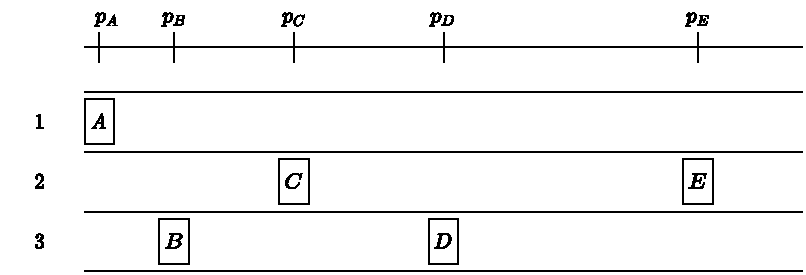
\includegraphics[width=0.7 \textwidth]{../figs/MLSL_simple}
\end{figure}
\pause
\begin{block}{$\mathcal{TS}$}
	$\mathcal{TS} \equiv (\mathbb{I}, \mathbb{L}, pos, vel, acc)$, where:
	\begin{align*}
	\mathbb{I} &\equiv \{A, B, C, D, E\}\\
	\mathbb{L} &\equiv \{1, 2, 3\}\\
	pos &\equiv \{A \mapsto p_A, \ldots, E \mapsto p_E \}\\
	vel &\ldots\\
	acc &\ldots
	\end{align*}
\end{block}




\end{frame}

\begin{frame}{Views}
Safety can be shown using only\textit{ local information}.\\
\bigskip
Restrict ourselves to subsets of continuous distance and contiguous lanes
\pause
\begin{figure}[h]
	\centering
	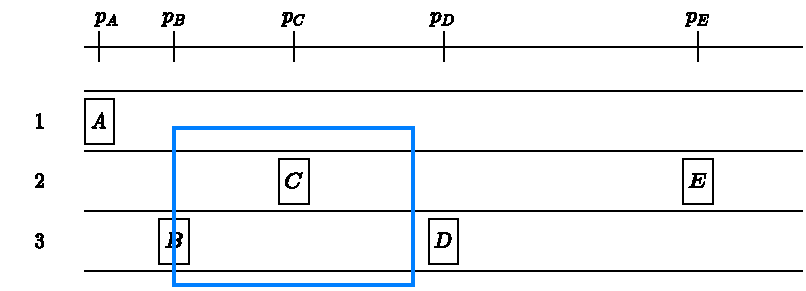
\includegraphics[width=0.7 \textwidth]{../figs/MLSL_simple_view}
\end{figure}

\pause
Given this view, $V$, the following formula holds:
\begin{equation*}
\mathcal{TS}, V \models \genfrac{}{}{0pt}{}{free\frown C \frown free}{B \frown free}
\end{equation*}

\end{frame}

\begin{frame}{Reservations}
Vehicles need more than a point to drive safety, they need a \textit{reservation}
\begin{figure}[h]
	\centering
	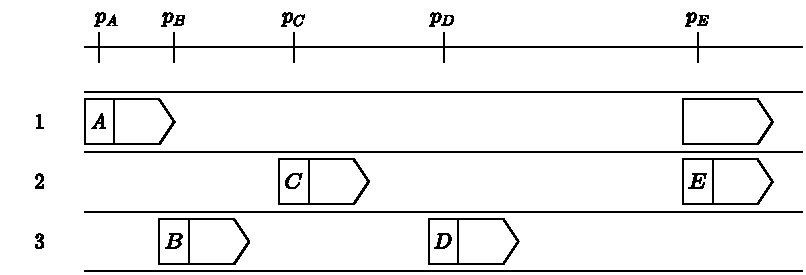
\includegraphics[width=0.7 \textwidth]{../figs/MLSL_reservation}
\end{figure}

Need two reservations when changing lanes
\pause
\begin{block}{$\mathcal{TS}$}
	$\mathcal{TS} \equiv (\mathbb{I}, \mathbb{L}, pos, vel, acc, res)$, where:
	\begin{equation*}
	res \equiv \{A\mapsto \{1\}, B \mapsto{\{3\}}, \ldots, E \mapsto \{1, 2\}\}
	\end{equation*}
\end{block}

\end{frame}

\begin{frame}{Claims}
Vehicles declare intent to change lanes through a \textit{claim}
\begin{figure}[h]
	\centering
	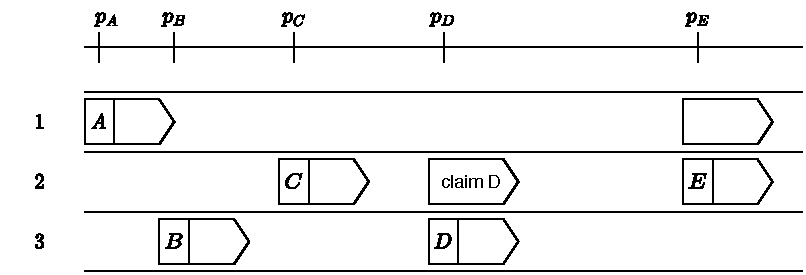
\includegraphics[width=0.7 \textwidth]{../figs/MLSL_claim}
\end{figure}
\pause
\begin{block}{$\mathcal{TS}$}
	$\mathcal{TS} \equiv (\mathbb{I}, \mathbb{L}, pos, vel, acc, res, clm)$, where:
	\begin{equation*}
	clm \equiv \{ * \mapsto \emptyset \} \oplus \{D \mapsto \{2\}\}
	\end{equation*}
\end{block}
\end{frame}

\begin{frame}{Standard view}
$V^s_{ego}$ is the \textit{standard view} with respect to a given vehicle.\\
\bigskip
Includes all lanes and a fixed interval before and after vehicle.
\pause
\begin{figure}[h]
	\centering
	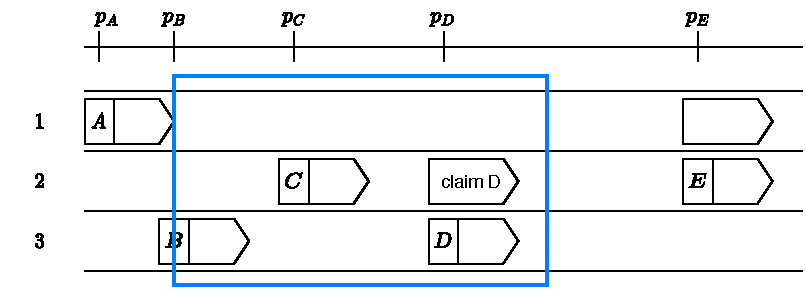
\includegraphics[width=0.7 \textwidth]{../figs/MLSL_standard_view}
\end{figure}
\pause
For the standard view with respect to $E$ we have:
\begin{equation*}
\mathcal{TS}, V^s_{C} \models \begin{matrix}free \\
											free \frown re(C) \frown free \frown cl(D) \frown free \\
											res(B) \frown free \frown re(D) \frown free \end{matrix}
\end{equation*}
\end{frame}

\begin{frame}{Safety goal}
The modality \textit{somwhere} $\varphi$:
\begin{equation*}
\langle \varphi \rangle \equiv true \frown \begin{pmatrix}true \\ \varphi \\ true\end{pmatrix} \frown true
\end{equation*}
\pause
\begin{block}{Global MLSL Safety}
Different vehicles do not reserve the same space:

\begin{equation*}
\mathcal{TS} \models \forall c, d: c \ne d \Rightarrow \neg \langle re(c) \land re(d)\rangle
\end{equation*}
\end{block}
\pause

\begin{block}{Local MLSL Safety}
Safety wrt arbitrary eqo vehicle
\begin{equation*}\label{eq:safety_goal}
\mathcal{TS}, V_{ego} \models \neg \exists c \neq ego \land \langle re(ego) \land re(c)\rangle
\end{equation*}
\end{block}
\end{frame}

\begin{frame}{Transitions}
Can change safety definition to:
\begin{equation*}\label{eq:safety_goal}
\mathcal{TS}, V_{ego} \models \neg \exists c \neq ego \land \langle re(ego) \land re(c)\rangle
\end{equation*}

\end{frame}

\begin{frame}{Controllers}
Created by using transition guards and state invariants.
\end{frame}

\begin{frame}{Proofs}
By induction on number of transitions to reach $\mathcal{TS}$

Assumptions

Boils down to proving
\end{frame}

\end{document}

